%% Fig 6 -- regenerated by LIEP-REGEN (owner's OK 2026-11-05; revised 2026-11-13: map -> fidelity curves, diagnostics removed, linear controls in (c); 2026-11-16: (c) each network at its rule, LIEP-6C: backprop with Muon, EP with Adam + cosine at kappa 0.1, lock-in with amplitude homeostasis; full grid in fig6c_appendix.tex). DRAFT caption for the owner to edit into the manuscript.
%% Graphic: regen/figures/src/fig6_basin.py, data and macros from regen/figures/export.py. Authored at 370.6 pt wide:
%% include with width=\textwidth and do not scale. Replaces fig1_basin.{pdf,tex}.
% generated by regen/figures/export.py -- do not edit
\newcommand{\FigKappa}{0.041}
\newcommand{\FigKappaLo}{0.025}
\newcommand{\FigKappaHi}{0.073}
\newcommand{\FigKappaN}{8}
\newcommand{\FigKappaTrained}{0.078}
\newcommand{\FigKappaRealInit}{0.089}
\newcommand{\FigBoundWp}{0.084}
\newcommand{\FigBoundWpLo}{0.018}
\newcommand{\FigBoundWpHi}{0.387}
\newcommand{\FigBoundSlope}{3.32}
\newcommand{\FigBoundN}{288}
\newcommand{\FigBoundTrainedWp}{0.076}
\newcommand{\FigBoundTrainedN}{72}
\newcommand{\FigEdgeLo}{0.5}
\newcommand{\FigEdgeHi}{1}
\newcommand{\FigProbeRandom}{0.862}
\newcommand{\FigCmpMeanRelu}{0.882}
\newcommand{\FigCmpMeanPhasorbp}{0.868}
\newcommand{\FigCmpMeanLockin}{0.854}
\newcommand{\FigCmpMeanCentred}{0.857}
\newcommand{\FigCmpNRelu}{20}
\newcommand{\FigCmpNPhasorbp}{20}
\newcommand{\FigCmpNLockin}{6}
\newcommand{\FigCmpNCentred}{6}
\newcommand{\FigEpsSpreadIn}{0.005}
\newcommand{\FigEpsSpreadOut}{0.16}
\newcommand{\FigLRPixels}{0.843}
\newcommand{\FigLRPhase}{0.862}
\newcommand{\FigProbeLockin}{0.880}
\newcommand{\FigProbeCentred}{0.877}
\newcommand{\FigProbePhasorbp}{0.886}
\newcommand{\FigBaseN}{3}
\newcommand{\FigCRelu}{0.893}
\newcommand{\FigCPhasorbp}{0.889}
\newcommand{\FigCLockin}{0.876}
\newcommand{\FigCCentred}{0.876}
\newcommand{\FigCProbePhasorbp}{0.892}
\newcommand{\FigCProbeLockin}{0.887}
\newcommand{\FigCProbeCentred}{0.888}
\newcommand{\FigCN}{6}


\begin{figure}[tbp]
\sffamily
\centering
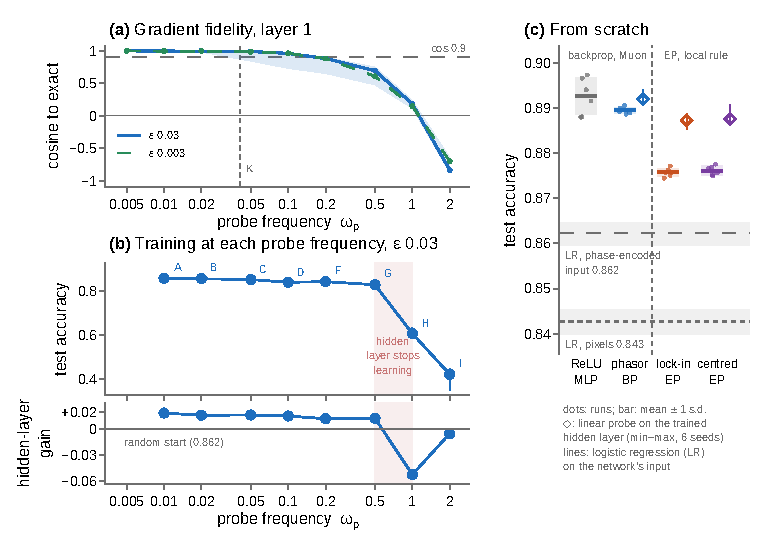
\includegraphics[width=\textwidth]{figures/fig6_basin.pdf}
\caption{Gradient fidelity and training across probe frequency, with the corrected lock-in.
\textbf{(a)} Median cosine between the layer-1 lock-in gradient and the exact gradient (implicit differentiation),
eight input draws per point, $n_\text{cycles}=4$, one warm-up cycle, at $\varepsilon=0.03$ (band: interquartile range)
and $\varepsilon=0.003$ (dashed). In this noiseless simulation fidelity does not depend on the probe amplitude: up to
$\omega_p=0.2$ the medians for $\varepsilon$ from 0.003 to 0.3 differ by at most \FigEpsSpreadIn{}; past it the
smallest amplitude falls lower (by up to \FigEpsSpreadOut). With noise, the smallest usable amplitude is set by the
noise (Figs~X--Y). Fidelity falls with $\omega_p$ near the slowest relaxation rate of the free settle,
$\kappa=\FigKappa$ (dotted; median over \FigKappaN{} draws, range \FigKappaLo--\FigKappaHi), and changes sign past $\omega_p\approx1$, where the response lags the probe by more than $90^\circ$.
\textbf{(b)} Training from scratch with lock-in EP at $\varepsilon=0.03$ and the marked $\omega_p$ (8 epochs, Adam
$\eta=3\times10^{-3}$): final test accuracy (top) and the gain of a linear probe on the hidden layer over the same
probe on the untrained network ($\FigProbeRandom$; bottom); median of three seeds (six at B), bars min--max.
Integrator step 0.1 during the gradient estimate from $\omega_p=0.2$ up, 0.5 below. Training hardly notices the loss
of gradient fidelity near $\kappa$: accuracy falls by about 0.02 up to G and the hidden layer keeps learning. Between
$\omega_p=\FigEdgeLo$ and \FigEdgeHi{} (shaded) the hidden layer stops learning and accuracy drops steeply.
\textbf{(c)} Training from scratch, 8 epochs, every run a point (\FigCN{} seeds per network), bar at the mean with a
$\pm1$ s.d.\ band; all scored on the 10,000 test images. The backprop networks are trained with the rule that gives
their best result, Muon (orthogonalised updates, tuned learning rate): a ReLU/softmax MLP 784--256--64--10 (median
\FigCRelu) and the phasor network by feedforward backprop (\FigCPhasorbp). The EP arms use a local rule, Adam with a
cosine learning-rate schedule (tuned), with layer 2's synapses held at $\kappa_2=0.1$ of their initial scale, which
weakens the top-down feedback that the settled network receives: lock-in EP with each output unit's drive amplitude
held by a local homeostatic loop (\FigCLockin) and centred EP with each row projected to its norm (\FigCCentred).
Diamonds: a linear probe on each phasor network's trained hidden layer (backprop \FigCProbePhasorbp, lock-in
\FigCProbeLockin, centred \FigCProbeCentred; median and range over the same runs). Lines: logistic regression on the
raw pixels (\FigLRPixels) and on the phase encoding the phasor network receives, as $(\cos\theta,\sin\theta)$
(\FigLRPhase); bands min--max over \FigBaseN{} seeds. Every network ends above both linear controls. Table~X gives every
network under each rule (constant Adam $10^{-3}$, Adam with cosine schedule, Muon), including EP trained with Muon.}
\label{fig:basin}
\end{figure}
